\documentclass[11pt]{article}
\usepackage[top=1.00in, bottom=1.0in, left=1.1in, right=1.1in]{geometry}
\usepackage{Sweave}
\renewcommand{\baselinestretch}{1.2}
\usepackage{graphicx}
\usepackage{natbib}
\usepackage{amsmath}
\usepackage{gensymb}
\usepackage{parskip}
\usepackage{hyperref}
\usepackage[utf8]{inputenc}

\def\labelitemi{--}
\parindent=0pt

\begin{document}

\renewcommand{\refname}{\CHead{}}




\newpage
{\bf Box. Growth, growing season length and the challenge of standardized metrics}
\begin{figure}[h!]
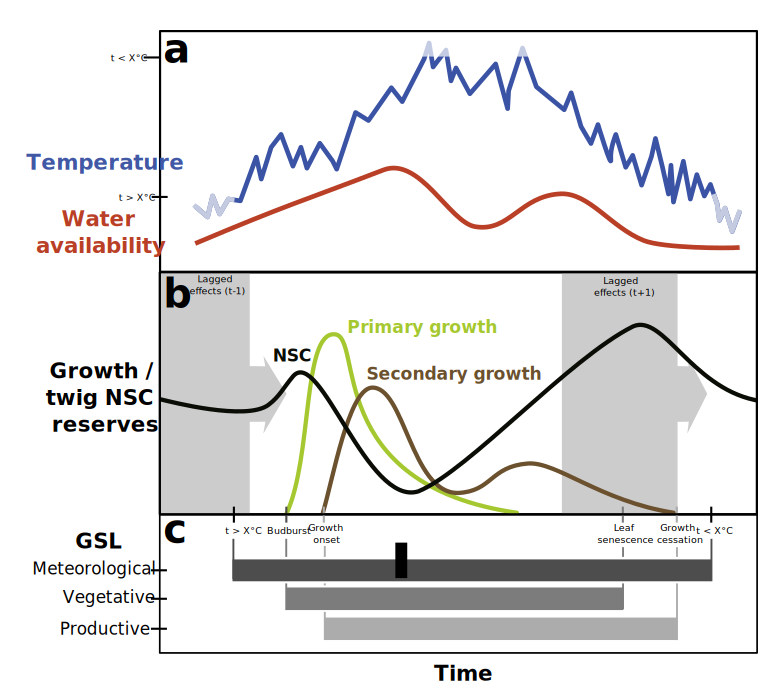
\includegraphics[width=0.95\textwidth]{..//figures/gslconcept/NEW_FI~1_ac_ver2.png}
\label{fig:defineGSLgrowth}
\end{figure}

A major challenge in determining how growth responds to longer growing seasons is the complexity of each, which means that neither can have one simple definition. Here we show the simplified climate of one year (a), which drives variation (b) in primary growth (root, shoot and leaf elongation) and secondary growth (radial wood growth), both of which often depend on growth from previous seasons. Each of these types of growth could define the growing season length (GSL, c) but similarly it can be defined meteorologically (e.g., days above 5\degree C with some level of soil moisture) or by large-scale measures of plant productivity \citep{korner2023four}. 

Of studies in our literature review, the largest proportion used metrics related to secondary growth, quantifying growth by measuring radial growth (e.g., through increment cores or dendrometers, $n=$28), but a number also looked at metrics related to primary growth, including C assimilation (e.g. net ecosystem productivity or gross primary productivity, $n=$20). A smaller number used metrics that reflect combined primary and secondary growth, including biomass, height, or number of stems ($n=$9), and root:shoot ratio ($n =$1). Some studies used modeled estimates of photosynthesis (e.g., \citet{smith2014implications} relied on daily photosynthesis estimates derived from the LPJ-GUESS photosynthesis model, while \citet{chen2000approaches} estimated photosynthese using the Integrated Terrestrial Ecosystem C-budget model, InTEC). 
Others measured photosynthesis at the leaf level, through flux towers, or used greenness metrics (NDVI). 

For growing season length, the largest number of studies used vegetative (e.g., budburst to leaf senescence in our figure above, 26 studies) or wood phenology 11 studies) as their definition, while a smaller number used a meteorological definitions or fixed dates (7 studies). We found 14 that did not directly measure GSL \citep[e.g.,][]{zhu2021different,dow2022warm,zohner2023effect}. Further, these definitions of GSL are simplified and could not be easily aligned, as we found 14 different metrics of start of season, 16 metrics of end of season (25 metrics of growing season length. See also `The challenge of metrics: Measuring growth and growing season length' in the Supplement. \\



{\Large {\bf Below from Supplement!}}

\section*{The challenge of metrics: Measuring growth and growing season length}

Understanding the diverse drivers and testing underlying hypotheses (Fig. \ref{fig:hypotheses}) for growth $\times$ season length relationships requires a common language. We found 14 different metrics of start of season, 16 metrics of end of season (25 metrics of growing season length), and 21 different metrics of growth across 59 studies---highlighting just part of the problem (see also \emph{Box: Growth, season length and the challenge of standardized metrics} in the main text). Definitions and metrics for external and internal drivers were myriad, %CJC 15Dec - I think we could again add numbers for external and internal divers, clarifying these were after systematically assigning studies into groups
with papers reporting dozens of tests of different aspects of climate over different temporal windows. Although this is understandable given the differing goals of these papers, it also slows progress. 

A common framework for explanatory and response variables would accelerate research by easing communication between fields and providing a path to comparable quantitative estimates. 
This should also include expected statistical tests, as we found a number of papers failed to directly test for growth $\times$ growing season length relationships (Fig. \ref{fig:heatmaps}), often instead testing only certain hypothesized indirect relationships \citep[e.g. spring temperature $\times$ growth in][]{dow2022warm}. % A first fundamental need for any framework is comparable quantitative estimates---which we currently lack. 

\subsection*{Measuring growth}

Tree growth can be defined and measured in a variety of ways. It is often divided into primary (growth from the root and shoot tips that results in increased height and length) versus secondary (growth that increases the thickness or girth of stems and branches above ground, as well as below ground parts), or leaf production versus wood production.  
Growth measurements vary across disciplines and study types, posing further challenges to an interdisciplinary approach to understanding how growing season length relates to growth. 
Greenhouse or growth chamber studies and provenance trials were more likely to measure height or biomass, whereas larger scale syntheses and remote-sensed studies are more likely to use metrics of carbon assimilation. 
The inconsistency of current metrics across fields is not surprising, but may be confusing-- including photosynthesis as a metric of growth may seem unconventional for ecophysiologists, for example, who may interpret the process of photosynthesis as distinct from growth-- and also stalls progress toward a unified model across disciplines.

Aligning across the range and scale of growth metrics will be critical for an integrated understanding of growth-growing season length relationships and implications under continued climate change.  
There is decoupling among some metrics of growth, as different types of growth (leaves, shoots, wood) have different phenologies within a season, and may vary across years, as well (e.g., with different lags, Fig. \ref{fig:gxelev}).
For example, vegetation photosynthesis may be poorly correlated with tree radial growth, and this relationship can vary seasonally \citep{cabon2022cross}. 
Further, tree radial growth is not a perfect indicator of whole tree growth, since plants allocate carbon to their roots, leaves, reproductive structures, and stores in addition to aboveground biomass. 
Relationships among different metrics of growth are not simple, so selecting relevant ones and aligning across the most widely used ones will be necessary, though not easy: the relationship  between photosynthesis, radial growth, and carbon uptake has large implications for future carbon sequestration and it remains widely debated \citep{green2022limits}. 
Further, there is a need to understand how to scale up across these varying metrics- from leaf and individual level to populations, communities, and ecosystems- while incorporating the variation that exists within and across levels.

\subsection*{Measuring growing season length}

Growing season length is defined in myriad ways due to varying definitions and metrics for the start of season and the end of season. For example, the end of season could be defined as budset, representing the end of vegetative phenology, or as xylogensis, representing the end of wood phenology. Additionally, several studies leveraged climate data as a proxy for start or end of season metrics, such as snowmelt for start of season or growing season GDDs. We therefore grouped all reported growing season length metrics into four separate categories: 1) `Climate and date' simulated by climate data, 2) `Vegetative phenology' through field observations or satellite derived measurements, 3) `Wood phenology' measured by dendrometers and xylogenesis, and 4) not measured, which includes all studies that only measured start or end of seasons but not both. 

Numerous studies in the review reported multiple metrics for end of season (e.g., budset versus leaf coloring) and found differing relationships between growth and growing season length depending on the end of season definition. We reported all combinations of assessments per study in our review. 

\section*{Extending disciplinary focus to help bridge the internal-external drivers divide} 

% Careful interdisciplinary is critical, but will benefit from shifts within disciplines. 
% Standardized measurements will not yield fully comparable estimates---especially on the relative impacts of external and internal drivers---without larger shifts within fields. We found that dendrochronology considers almost exclusively external climatic drivers, while physiological tests of internal constraints do not usually make predictions that scale up easily beyond the lab or greenhouse. Major fields studying this relationship---dendrochronology, phenology research and physiology---all need to broaden in specific ways to overlap with one another to facilitate interdisciplinary work. At the same time, all fields have missed certain major hypotheses they could test (Fig. \ref{fig:hypotheses}), highlighting the need to integrate perspectives from other disciplines with relevant theory and methods. 

Each field studying growth $\times$ growing season length today has its own historical aims, and thus, its own biases towards certain species, methods and metrics. For example, dendrochronology's original focus on using tree growth to estimate climate has led to sampling biases \citep[e.g. to `climate-sensitive' individual trees,][]{klesse2018sampling,nehrbass2014influence} and statistical detrending \citep{rollinson2021climate}, which may obscure patterns where the signal of longer growing seasons and biotic drivers may be most apparent (such as rapid growth phases). Dendrochronology also generally focuses on conifers \citep[gymnosperms,][]{zhao2019international}, creating a major split from most studies of leaf phenology, which focus almost entirely on deciduous angiosperm species (see Fig. \ref{fig:itrbdpep}). By contrast, phenology research has been strongly focused on spring events (e.g. budburst, leafout), with limited data on fall events and thus limited data to calculate growing season length. This focus on spring events may have been justified decades ago, when most shifts from anthropogenic warming occurred in the spring, but less justified as increasing research suggests important complexity in fall shifts \citep{gill2015,zohner2023effect} and a need to scale up phenological research to understand tree growth.

\clearpage
\section{References}
\bibliography{..//bibtex/grephonbib}
\bibliographystyle{/Users/Lizzie/Documents/git/bibtex/styles/besjournals.bst} % pnas.bst says 87 refs on 18 May 2024


\end{document}
